%%%%%%%%%%%%%%%%%%%%%%%%%%%%%%%% Introducción:
\begin{frame}[plain]
  \begin{figure}
    Un conjunto de datos agrupados en $k$ grupos ``similares''.
    \centering
    \begin{subfigure}[b]{0.6\textwidth}
      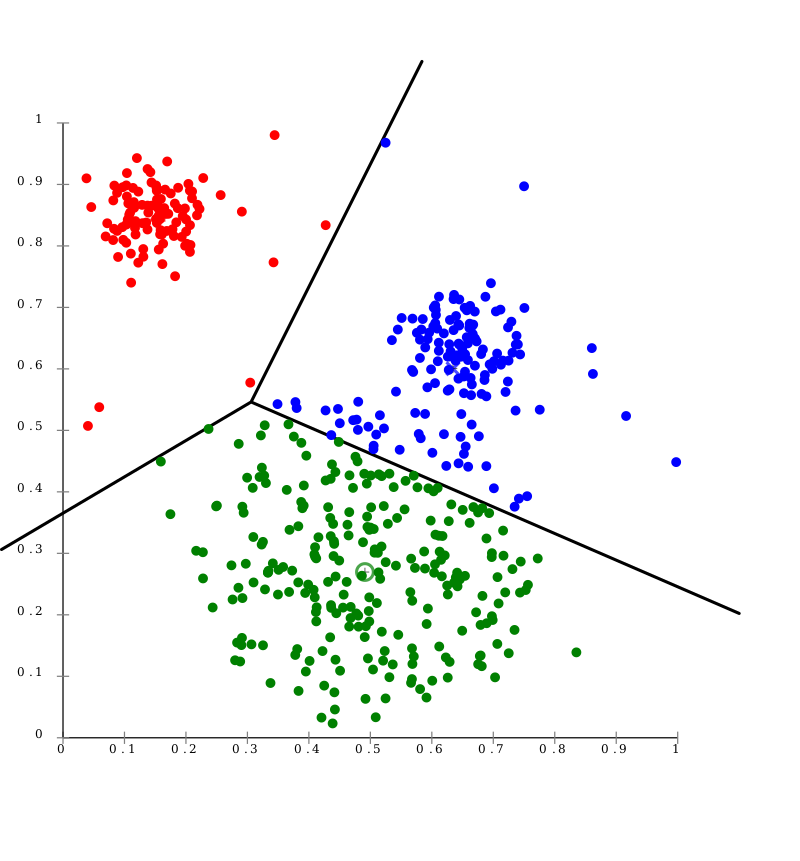
\includegraphics[width=\textwidth]{./Imagenes/k-means.png}
      \caption*{Agrupamiento por K-means.}
    \end{subfigure}
  \end{figure}
  \textbf{¿Cómo agrupar? ...}
\end{frame}
